\documentclass{exercise}

\institute{Lehr- und Forschungsgebiet Kontinuumsmechanik}
\title{Übung 4}
\author{Joshua Feld, 406718}
\course{Mechanik verformbarer Körper}
\professor{Itskov}
\semester{Sommersemester 2022}
\program{CES (Bachelor)}

\begin{document}
    \maketitle


    \section*{Aufgabe 1}

    \begin{problem}
        Für zwei verschiedene Belastungsfälle eines Bauteils sind die Spannungszustände bekannt:
        \begin{enumerate}[label=(\roman*)]
            \item \(\sigma_{x, 1}, \sigma_{y, 1}, \tau_{xy, 1}\)
            \item \(\sigma_u, \sigma_v, \tau_{uv}\)
        \end{enumerate}
        Es sind für den Fall, dass beide Belastungen gleichzeitig wirken, zu berechnen:
        \begin{enumerate}
            \item die Spannungen \(\sigma_{x, \text{ges}}\), \(\sigma_{y, \text{ges}}\) und \(\tau_{xy, \text{ges}}\),
            \item die Hauptnormalspannungen \(\sigma_{1, 2}\),
            \item die Hauptschubspannungen \(\tau_{\text{max}}\) und
            \item die Hauptnormal- und Hauptschubspannungsrichtungen.
        \end{enumerate}
        Gegeben:
        \begin{enumerate}[label=(\roman*)]
            \item \(\sigma_{x, 1} = -460\sis{\newton\per\milli\meter\squared}, \sigma_{y, 1} = 140\sis{\newton\per\milli\meter\squared}, \tau_{xy, 1} = 0\sis{\newton\per\milli\meter\squared}\)
            \item \(\sigma_u = 770\sis{\newton\per\milli\meter\squared}, \sigma_v = 230\sis{\newton\per\milli\meter\squared}, \tau_{uv} = -162\sis{\newton\per\milli\meter\squared}, \varphi = 30^\circ\)
        \end{enumerate}
    \end{problem}

    \subsection*{Lösung}
    Das Superpositionsprinzip von Kräften besagt, dass wenn auf einen Punkt (Massenpunkt, auch starren Körper) mehrere Kräfte \(\bm{F}_1, \ldots, \bm{F}_n\) wirken, sich diese vektoriell zu einer resultierenden Kraft \(\bm{F}_{\text{res}} = \sum_{i = 1}^n\bm{F}_i\) aufaddieren.
    Das heißt, dass \(\bm{F}_{\text{res}}\) dieselbe Wirkung hat, wie sämtliche Kräfte \(\bm{F}_1, \ldots, \bm{F}_n\) gemeinsam.
    \begin{enumerate}
        \item Es werden die Spannungen des \(u\)-\(v\)-Systems in das \(x\)-\(y\)-System transformiert.
        Unter Zuhilfenahme der Transformationsgleichungen ergeben sich die Spannungen
        \[
            \sigma_{u \to x} = 775,3\sis{\newton\per\milli\meter\squared}, \quad \sigma_{v \to y} = 224,7\sis{\newton\per\milli\meter\squared}, \quad \tau_{uv \to xy} = 152,8\sis{\newton\per\milli\meter\squared}.
        \]
        Die Superposition der Spannungen ergibt
        \begin{align*}
            \sigma_{x, \text{ges}} &= \sigma_{x, 1} + \sigma_{u \to x} = 315,3\sis{\newton\per\milli\meter\squared},\\
            \sigma_{y, \text{ges}} &= \sigma_{y, 1} + \sigma_{v \to y} = 364,7\sis{\newton\per\milli\meter\squared},\\
            \tau_{xy, \text{ges}} &= \tau_{xy, 1} + \tau_{uv \to xy} = 152,8\sis{\newton\per\milli\meter\squared}.
        \end{align*}
        Ausgehend von diesem gesamten Spannungszustand lassen sich die weiteren Aufgabenteile wie gewohnt lösen.
        \item
        \[
            \sigma_1 = 494,8\sis{\newton\per\milli\meter\squared}, \quad \sigma_2 = 185,2\sis{\newton\per\milli\meter\squared}.
        \]
        \item
        \[
            \tau_{\text{max}} = 154,8\sis{\newton\per\milli\meter\squared}.
        \]
        \item
        \[
            \varphi^* = 49,6^\circ, \quad \varphi^{**} = 4,6^\circ.
        \]
    \end{enumerate}


    \section*{Aufgabe 2}

    \begin{problem}
        In einem Punkt eines Körpers seien die Komponenten des Cauchy'schen Spannungstensors \(\sigma\) in kartesischen Koordinaten gegeben.
        \begin{enumerate}
            \item Berechnen Sie den Spannungsvektor \(\bm{t}\) auf einer Schnittfläche mit dem Normalenvektor \(\bar{\bm{n}}\).
            \item Welchen Betrag hat der Spannungsvektor?
            \item Wie groß sind die Normalspannung \(\sigma_N\) und der Schubspannungsvektor \(\bm{\tau}\)?
            \item Welcher Winkel wird von \(\bm{t}\) und \(\bar{\bm{n}}\) eingeschlossen?
        \end{enumerate}
        Gegeben: \(\sigma = \begin{pmatrix}
            9 & -3 & 0\\
            -3 & -9 & 0\\
            0 & 0 & 3
        \end{pmatrix}\sis{\mega\pascal}, \bar{\bm{n}} = \begin{pmatrix}
            2\\
            -2\\
            1
        \end{pmatrix}\)
    \end{problem}

    \subsection*{Lösung}
    \begin{enumerate}
        \item Für die nachfolgenden Berechnungen muss der Normalenvektor der Fläche ein Einheitsvektor sein (d.h. die Länge muss \(1\) sein), um eine Skalierung der Spannungen zu vermeiden.
        Der in der Aufgabenstellung angegebene Vektor \(\bar{\bm{n}}\) liegt nicht als Einheitsvektor vor.
        Der in die selbe Richtung zeigende Einheitsvektor \(\bm{n}\) ergibt sich zu
        \[
            \bm{n} = \frac{\bar{\bm{n}}}{\norm*{\bar{\bm{n}}}} = \frac{\bar{\bm{n}}}{\sqrt{2^2 + \parentheses*{-2}^2 + 1^2}} = \frac{\bar{\bm{n}}}{3} = \begin{pmatrix}
                \frac{2}{3}\\
                -\frac{2}{3}\\
                \frac{1}{3}
            \end{pmatrix}.
        \]
        Mithilfe des Cauchy Satzes folgt für den Spannungsvektor
        \[
            \bm{t} = \sigma\bm{n} = \begin{pmatrix}
                9 & -3 & 0\\
                -3 & -9 & 0\\
                0 & 0 & 3
            \end{pmatrix}\begin{pmatrix}
                \frac{2}{3}\\
                -\frac{2}{3}\\
                \frac{1}{3}
            \end{pmatrix}\sis{\mega\pascal} = \begin{pmatrix}
                8\\
                4\\
                1
            \end{pmatrix}\sis{\mega\pascal}
        \]
        \item
        \[
            \norm*{\bm{t}} = \sqrt{8^2 + 4^2 + 1^2} = 9.
        \]
        \item Der Spannungsvektor \(\bm{t}\) lässt sich vektoriell in eine Normalspannung \(\sigma_N\) und einen Schubspannungsvektor \(\bm{\tau}\) zerlegen.
        Hierbei ist die Normalspannung eine skalare Größe, die in Richtung des Normalenvektors wirkt.
        Es gilt
        \[
            \bm{t} = \bm{\tau} + \sigma_N\bm{n}.
        \]
        Die Normalspannung ergibt sich zu
        \[
            \sigma_n = \bm{t} \cdot \bm{n} = \begin{pmatrix}
                8\\
                4\\
                1
            \end{pmatrix} \cdot \begin{pmatrix}
                \frac{2}{3}\\
                -\frac{2}{3}\\
                \frac{1}{3}
            \end{pmatrix}\sis{\mega\pascal} = 3\sis{\mega\pascal},
        \]
        wodurch Folgendes gilt:
        \[
            \bm{\tau} = \bm{t} - \sigma_N\bm{n} = \begin{pmatrix}
                6\\
                6\\
                0
            \end{pmatrix}\sis{\mega\pascal}.
        \]
        \item Aus der Definition des Skalarproduktes
        \[
            \bm{t} \cdot \bm{n} = \norm*{t} \cdot \norm*{n} \cdot \cos\varphi,
        \]
        folgt für den Winkel \(\varphi\) zwischen den beiden Vektoren
        \[
            \varphi = \arccos\frac{\bm{t} \cdot \bm{n}}{\norm*{\bm{t}} \cdot \norm*{\bm{n}}} = \arccos\frac{\sigma_N}{9 \cdot 1} = \arccos\frac{1}{3} = 70,53^\circ.
        \]
    \end{enumerate}


    \section*{Aufgabe 3}

    \begin{problem}
        In der experimentellen Mechanik werden Dehnungsmessstreifen (DMS) zur Ermittlung der Spannungen (auf der Oberfläche) eines bekannten Materials eingesetzt.
        Mit einer \(45^\circ\) Rosette werden die Dehnungen \(\varepsilon_a\), \(\varepsilon_b\) und \(\varepsilon_c\) gemessen.
        \begin{center}
            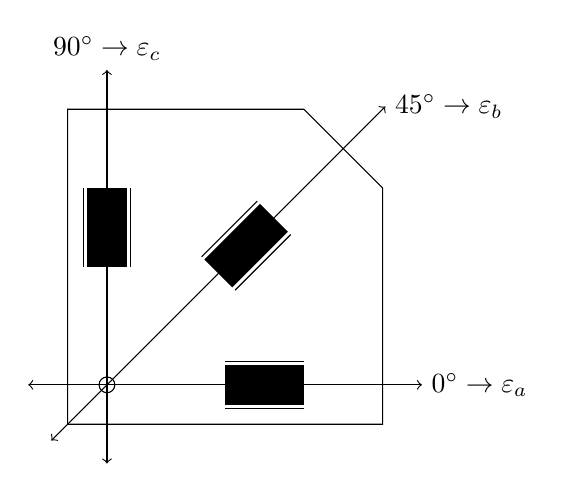
\begin{tikzpicture}
                \draw[<->] (-1,0) -- (4,0) node[right] {\(0^\circ \to \varepsilon_a\)};
                \fill (1.5,-.25) rectangle (2.5,.25);
                \draw (1.5,-.3) -- (2.5,-.3);
                \draw (1.5,.3) -- (2.5,.3);
                \begin{scope}[rotate=45]
                    \draw[<->] (-1,0) -- (5,0) node[right] {\(45^\circ \to \varepsilon_b\)};
                    \fill (2,-.25) rectangle (3,.25);
                    \draw (2,-.3) -- (3,-.3);
                    \draw (2,.3) -- (3,.3);
                \end{scope}
                \draw[<->] (0,-1) -- (0,4) node[above] {\(90^\circ \to \varepsilon_c\)};
                \fill (-.25,1.5) rectangle (.25,2.5);
                \draw (-.3,1.5) -- (-.3,2.5);
                \draw (.3,1.5) -- (.3,2.5);
                \draw (0,0) circle (1mm);
                \draw (-.5,-.5) -- (-.5,3.5) -- (2.5,3.5) -- (3.5,2.5) -- (3.5,-.5) -- cycle;
            \end{tikzpicture}
        \end{center}
        Berechnen Sie die Hauptspannungen sowie die Hauptdehnungsrichtungen.

        Gegeben: \(\varepsilon_a = 60 \cdot 10^{-5}, \varepsilon_b = 75 \cdot 10^{-5}, \varepsilon_c = -40 \cdot 10^{-5}\)
    \end{problem}

    \subsection*{Lösung}
    Der Dehnungszustand im \(a\)-\(c\)-Koordinatensystem und der Dehnungszustand in dem \(45^\circ\) dazu gedrehten Koordinatensystem sind nicht vollständig gegeben.
    Daher muss vor der Berechnung der Hauptdehnungen der Dehnungszustand in einem der beiden Koordinatensysteme vollständig beschrieben werden.
    Wir definieren das \(x\)-\(y\)-Koordinatensystem wie das \(a\)-\(c\)-Koordinatensystem und das \(\xi\)-\(\eta\)-Koordinatensystem um \(45^\circ\) dazu gedreht.

    Zusammenfassend ist folgendes gegeben:
    \begin{center}
        \begin{tabular}{cc}
            \toprule
            \(x\)-\(y\) & \(\xi\)-\(\eta\)\\
            \midrule
            \(\varepsilon_x = \varepsilon_a\) & \(\varepsilon_\xi = \varepsilon_b\)\\
            \(\varepsilon_y = \varepsilon_c\) & \(\varepsilon_\eta = ?\)\\
            \(\gamma_{xy} = ?\) & \(\gamma_{\xi\eta} = ?\)\\
            \bottomrule
        \end{tabular}
    \end{center}
    Mittels der Invariantenbeziehung
    \[
        \varepsilon_a + \varepsilon_y = \varepsilon_\xi + \varepsilon_\eta
    \]
    lässt sich \(\varepsilon_\eta = -55 \cdot 10^{-5}\) leicht ermitteln.
    Mithilfe der Transformationsgleichungen
    \begin{align*}
        \varepsilon_\xi = \frac{1}{2}\parentheses*{\varepsilon_x + \varepsilon_y} + \frac{1}{2}\parentheses*{\varepsilon_x - \varepsilon_y}\cos\parentheses*{2\varphi} + \frac{1}{2}\gamma_{xy}\sin\parentheses*{2\varphi},\\
        \varepsilon_\eta = \frac{1}{2}\parentheses*{\varepsilon_x + \varepsilon_y} - \frac{1}{2}\parentheses*{\varepsilon_x - \varepsilon_y}\cos\parentheses*{2\varphi} - \frac{1}{2}\gamma_{xy}\sin\parentheses*{2\varphi},\\
        \frac{1}{2}\gamma_{\xi\eta} = -\frac{1}{2}\parentheses*{\varepsilon_x - \varepsilon_y}\sin\parentheses*{2\varphi} + \frac{1}{2}\gamma_{xy}\cos\parentheses*{2\varphi}
    \end{align*}
    und dem Winkel \(\varphi = 45^\circ\) lässt sich \(\gamma_{xy} = 130 \cdot 10^{-5}\) bestimmen.
    Somit ist der Zustand im \(x\)-\(y\)-Koordinatensystem vollständig beschrieben und dient fortan als Referenz.
    Die Formel für die Hauptdehnungen
    \[
        \varepsilon_{1, 2} = \frac{\varepsilon_x + \varepsilon_y}{2} \pm \sqrt{\parentheses*{\frac{\varepsilon_x - \varepsilon_y}{2}}^2 + \parentheses*{\frac{1}{2}\gamma_{xy}}^2}
    \]
    und die Formel für die Hauptdehnungsrichtung
    \[
        \varphi = \frac{1}{2}\arctan\frac{\gamma_{xy}}{\varepsilon_x - \varepsilon_y}
    \]
    liefern die Ergebnisse
    \[
        \varepsilon_1 = 92,01 \cdot 10^{-5}, \quad \varepsilon_2 = -72,01 \cdot 10^{-5}, \quad \varphi = 26,22^\circ.
    \]


    \section*{Aufgabe 4}

    \begin{problem}
        Für die Ermittlung der Werkstoffkennwerte Elastizitätsmodul \(E\) und Querkontraktionszahl \(\nu\) wird eine Blechprobe im Zugversuch untersucht.
        Die unten aufgeführten Spannungen und Abmessungen sind im unbelasteten (Index \(0\)) bzw. belasteten (Index \(1\)) Zustand gemessen worden.
        \begin{center}
            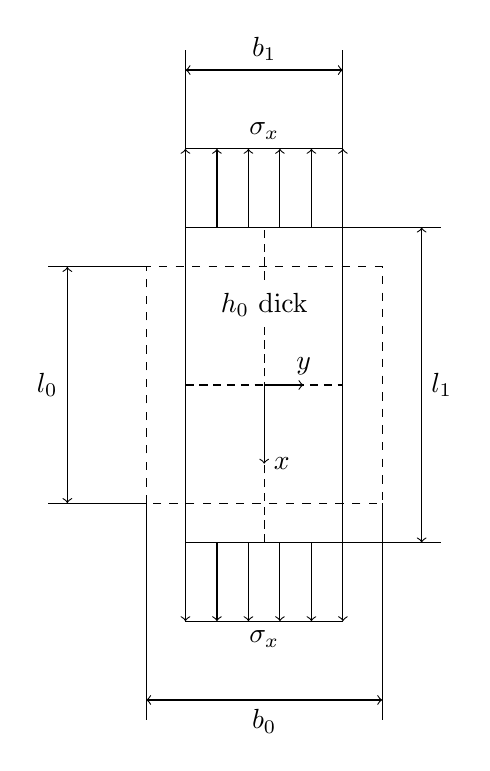
\begin{tikzpicture}
                \draw (0,0) rectangle (2,4);
                \draw[dashed] (-.5,.5) rectangle (2.5,3.5);
                \draw[densely dashed] (1,0) -- (1,4);
                \draw[densely dashed] (0,2) -- (2,2);
                \draw[->] (1,2) -- (1.5,2) node[above] {\(y\)};
                \draw[->] (1,2) -- (1,1) node[right] {\(x\)};
                \foreach \i in {0,0.4,...,2}
                {
                    \draw[->] (\i,0) -- (\i,-1);
                    \draw[->] (\i,4) -- (\i,5);
                }
                \draw (0,-1) -- (2,-1) node[midway,below] {\(\sigma_x\)};
                \draw (0,5) -- (2,5) node[midway,above] {\(\sigma_x\)};
                \draw (-.5,.5) -- (-.5,-2.25);
                \draw (2.5,.5) -- (2.5,-2.25);
                \draw[<->] (-.5,-2) -- (2.5,-2) node[midway,below] {\(b_0\)};
                \draw (0,4) -- (0,6.25);
                \draw (2,4) -- (2,6.25);
                \draw[<->] (0,6) -- (2,6) node[midway,above] {\(b_1\)};
                \draw (-.5,.5) -- (-1.75,.5);
                \draw (-.5,3.5) -- (-1.75,3.5);
                \draw[<->] (-1.5,.5) -- (-1.5,3.5) node[midway,left] {\(l_0\)};
                \draw (2,0) -- (3.25,0);
                \draw (2,4) -- (3.25,4);
                \draw[<->] (3,0) -- (3,4) node[midway,right] {\(l_1\)};
                \node[fill=white,anchor=south] at (1,2.75) {\(h_0\) dick};
            \end{tikzpicture}
        \end{center}
        Berechnen Sie E-Modul und Querkontraktionszahl der Probe.

        Gegeben:
        \begin{align*}
            \sigma_{x, 0} &= 0\sis{\newton\per\milli\meter\squared}, & b_0 &= 30,012\sis{\milli\meter}, & l_0 &= 100,17\sis{\milli\meter}, & h_0 &= 1\sis{\milli\meter},\\
            \sigma_{x, 1} &= 200\sis{\newton\per\milli\meter\squared}, & b_1 &= 29,971\sis{\milli\meter}, & l_1 &= 100,66\sis{\milli\meter}
        \end{align*}
    \end{problem}

    \subsection*{Lösung}
    Die Querkontraktion \(\nu\) ist das Verhältnis von zwei orthogonalen Dehnungen:
    \[
        \nu = -\frac{\varepsilon_y}{\varepsilon_x}, \quad \nu = -\frac{\varepsilon_z}{\varepsilon_x}.
    \]
    Mit den Dehnungen
    \[
        \varepsilon_x = \frac{\Delta l}{l_0} = \frac{l_1 - l_0}{l_0} = \frac{7}{1431}, \quad \varepsilon_y = \frac{\Delta b}{b_0} = \frac{b_1 - b_0}{b_0} = -\frac{1}{732}
    \]
    folgt direkt
    \[
        \nu = -\frac{\varepsilon_y}{\varepsilon_x} = \frac{477}{1708} = 0,2793.
    \]
    Das E-Modul folgt direkt aus dem Hook'schen Gesetz für uniaxiale Dehnung
    \[
        E = \frac{\sigma_{x, 1}}{\varepsilon_x} = 40885,71\sis{\mega\pascal}.
    \]


    \section*{Aufgabe 5}

    \begin{problem}
        Bei der Belastung eines isotropen, homogenen und linear-elastischen Materials unter isothermen Bedingungen wurden die Deformationen \(\varepsilon_x\), \(\varepsilon_y\) und \(\gamma_{xy}\) gemessen.
        Es liege ein ebener Spannungszustand vor (\(\sigma_z = 0\)).
        Das Material ist durch den Elastizitätsmodul \(E\) und die Querkontraktionszahl \(\nu\) charakterisiert.
        Berechnen Sie
        \begin{enumerate}
            \item den Spannungszustand in der \(xy\)-Ebene,
            \item die Dehnung \(\varepsilon_z\),
            \item die Hauptspannungen und deren Richtungen,
            \item die Hauptschubspannungen, deren Richtungen sowie die zugehörigen Normalspannungen.
        \end{enumerate}
        Gegeben: \(\varepsilon_x = 0,1, \varepsilon_y = 0,05, \gamma_{xy} = 0,15, E = 2,1 \cdot 10^5\sis{\newton\per\milli\meter\squared}, \nu = 0,3\)
    \end{problem}

    \subsection*{Lösung}
    \begin{enumerate}
        \item Aus dem verallgemeinerten Hook'schen Gesetz
        \begin{align*}
            \varepsilon_x &= \frac{1}{E}\parentheses*{\sigma_x - \nu\parentheses*{\sigma_y + \sigma_z}} + \alpha_T\Delta T,\\
            \varepsilon_y &= \frac{1}{E}\parentheses*{\sigma_y - \nu\parentheses*{\sigma_x + \sigma_z}} + \alpha_T\Delta T,\\
            \varepsilon_z &= \frac{1}{E}\parentheses*{\sigma_z - \nu\parentheses*{\sigma_x + \sigma_y}} + \alpha_T\Delta T,
        \end{align*}
        folgt mit \(\sigma_z = 0\) und \(\Delta T = 0\)
        \[
            \varepsilon_x = \frac{1}{E}\parentheses*{\sigma_x - \nu\sigma_y}, \quad \varepsilon_x = \frac{1}{E}\parentheses*{\sigma_y - \nu\sigma_x}, \quad \varepsilon_x = -\frac{\nu}{E}\parentheses*{\sigma_x - \nu\sigma_y}
        \]
        beziehungsweise
        \begin{align*}
            \sigma_x &= E\varepsilon_x + \nu\sigma_y = 2,654 \cdot 10^4\sis{\newton\per\milli\meter\squared},\\
            \sigma_y &= E\varepsilon_y + \nu\sigma_x = 1,846 \cdot 10^4\sis{\newton\per\milli\meter\squared}.
        \end{align*}
        Mit dem Schubmodul
        \[
            G = \frac{E}{2\parentheses*{1 + \nu}}
        \]
        folgt
        \[
            \tau_{xy} = G\gamma_{xy} = 1,21 \cdot 10^4\sis{\newton\per\milli\meter\squared}.
        \]
        \item
        \[
            \varepsilon_z = -\frac{\nu}{E}\parentheses*{\sigma_x + \sigma_y} = -0,0643
        \]
        \item Aus
        \[
            \sigma_{1, 2} = \frac{\sigma_x + \sigma_y}{2} \pm \sqrt{\parentheses*{\frac{\sigma_x - \sigma_y}{2}}^2 + \tau_{xy}^2}, \quad \tan\parentheses*{2\varphi^*} = \frac{2\tau_{xy}}{\sigma_x - \sigma_y}
        \]
        folgt direkt
        \[
            \sigma_1 = 3,526 \cdot 10^4\sis{\newton\per\milli\meter\squared}, \quad \sigma_2 = 9,743 \cdot 10^3\sis{\newton\per\milli\meter\squared}, \quad \varphi^* = 35,77^\circ.
        \]
        Zuordnen des Winkels zu den Hauptspannungen liefert
        \[
            \varphi_1^* = 35,77^\circ, \quad \varphi_2^* = 125,77^\circ.
        \]
        \item Es gilt
        \[
            \tau_{\text{max}} = \pm\sqrt{\parentheses*{\frac{\sigma_x - \sigma_y}{2}}^2 + \tau_{xy}^2} = \pm 1,276 \cdot 10^4\sis{\newton\per\milli\meter\squared}.
        \]
        Der Zusammenhang zwischen den Winkeln liefert
        \[
            \varphi_1^{**} = \varphi_1^* + 45^\circ = 80,77^\circ, \quad \varphi_2^{**} = \varphi_2^* + 45^\circ = 170,77^\circ.
        \]
        Durch die Invariantenbeziehung folgt
        \[
            \sigma_M = \frac{1}{2}\parentheses*{\sigma_1 + \sigma_2} = \frac{1}{2}\parentheses*{\sigma_x + \sigma_y} = 2,25 \cdot 10^4\sis{\newton\per\milli\meter\squared}.
        \]
    \end{enumerate}


    \section*{Aufgabe 6}

    \begin{problem}
        Ein Bauteil besteht aus einem Vollzylinder (Durchmesser \(d\)), der sich spielfrei in einem Hohlzylinder (Außendurchmesser \(D\)) befindet.
        Beide Zylinder haben die gleiche Länge \(L\).
        Sie befinden sich zwischen zwei starren Platten und werden mit der Kraft \(F\) belastet.
        \begin{enumerate}
            \item Welche Kräfte und Spannungen wirken in den Zylindern?
            \item Wie groß ist die Längenänderung?
        \end{enumerate}
        Gegeben: \(E_{\text{voll}} = 2,1 \cdot 10^5\sis{\newton\per\milli\meter\squared}, E_{\text{hohl}} = 1,15 \cdot 10^5\sis{\newton\per\milli\meter\squared}, d = 100\sis{\milli\meter}, D = 200\sis{\milli\meter}, l = 200\sis{\milli\meter}\), \(F = 400\sis{\kilo\newton}\)
    \end{problem}

    \subsection*{Lösung}
    \begin{enumerate}
        \item Das Kräftegleichgewicht in \(\uparrow\)-Richtung
        \[
            F + F_{\text{hohl}} + F_{\text{voll}} = 0
        \]
        liefert eine GLeichung und zwei Unbekannte.
        Das System ist somit einfach statisch unbestimmt.
        Mit der Verträglichkietsbedingung \(\Delta l = \Delta l_{\text{voll}} = \Delta l_{\text{hohl}}\) und dem Hook'schen Gesetz
        \[
            F = \frac{EA}{l_0}\Delta l
        \]
        folgt
        \[
            \frac{F_{\text{voll}}}{A_{\text{voll}}E_{\text{voll}}} = \frac{F_{\text{hohl}}}{A_{\text{hohl}}E_{\text{hohl}}} \iff F_{\text{hohl}} = \frac{A_{\text{hohl}}E_{\text{hohl}}}{A_{\text{voll}}E_{\text{voll}}}F_{\text{voll}}.
        \]
        In das Kräftegleichgewicht eingesetzt folgt mit den Flächen
        \[
            A_{\text{hohl}} = \frac{\pi}{4}\parentheses*{D^2 - d^2} = 23561,94\sis{\milli\meter\squared}, \quad A_{\text{voll}} = \frac{\pi}{4}d^2 = 7853,98\sis{\milli\meter\squared}
        \]
        somit
        \[
            F_{\text{hohl}} = -\frac{F}{1 + \frac{A_{\text{voll}}E_{\text{voll}}}{A_{\text{hohl}}E_{\text{hohl}}}} = -248,649\sis{\kilo\newton}, \quad F_{\text{voll}} = -\frac{F}{1 + \frac{A_{\text{hohl}}E_{\text{hohl}}}{A_{\text{voll}}E_{\text{voll}}}} = -151,351\sis{\kilo\newton}.
        \]
        Für die Spannungen ergibt sich
        \[
            \sigma_{\text{hohl}} = \frac{F_{\text{hohl}}}{A_{\text{hohl}}} = -10,55\sis{\mega\pascal}, \quad \sigma_{\text{voll}} = \frac{F_{\text{voll}}}{A_{\text{voll}}} = -19,27\sis{\mega\pascal}.
        \]
        \item Die Längenänderung ergibt sich aus dem Hook'schen Gesetz wie folgt:
        \[
            \Delta l = \Delta l_{\text{hohl}} = \frac{lF_{\text{hohl}}}{E_{\text{hohl}}A_{\text{hohl}}} = 18,35 \cdot 10^{-3}\sis{\milli\meter}.
        \]
    \end{enumerate}
\end{document}
